\chapter{Results}
\label{chap:results}


All results are obtained on a PC with an AMD FX-9590, 16 GB RAM and an AMD Radeon HD 7970. 


\section{Shape Detection Benchmarking}

This interactions proposes in this thesis heavily rely on the ability to detect meaningful shapes for regions of interest within interactive time. 


\subsection{Errors and Crap}

A problem with the shape detection implementation by Schnabel et. al\cite{schnabel-2007-software} are reoccurring non-terminations for some octree nodes, causing the shape detection coroutine to stall. To circumvent this problem, all shape detection tasks that are dispatched to the \verb|sequential computation applicator| are assigned a timeout value of one second, after which the computation is interrupted. 
\\
Another reoccurring problem with the shape detection are plausible shapes. The RANSAC options guarantee that shapes are found that fit the local geometry within a certain margin, $\alpha$ for the normal's angle and $\epsilon$ for the distance the the shape. So within theses two parameters, the shape is considered to be valid. However, certain constellation of points allow the shape detection to produce non-plausible results that valid in terms of the RANSAC shape detection, but are not plausible to the eye. A prominent example is a torus that is fitted onto a section that clearly describes a cylinder. The major radius of the torus is at such dimensions that the local cylinder fits within the curvature of the torus, thus a torus is detected, rather than the simpler cylinder. Figure \ref{fig:missfittedTorus} shows this behavior within an example scene that consists multiple primitives. Figure \ref{fig:missfittedTorus2} shows the size of the detected torus. 
\\
The reason that allows this non-plausibility of the shape is due to the density controlling the $\epsilon$ parameter, weakening the margin for octree nodes of larger volume. 


\begin{figure}
\centering
\subcaptionbox{ \label{fig:missfittedTorus1}}{%
  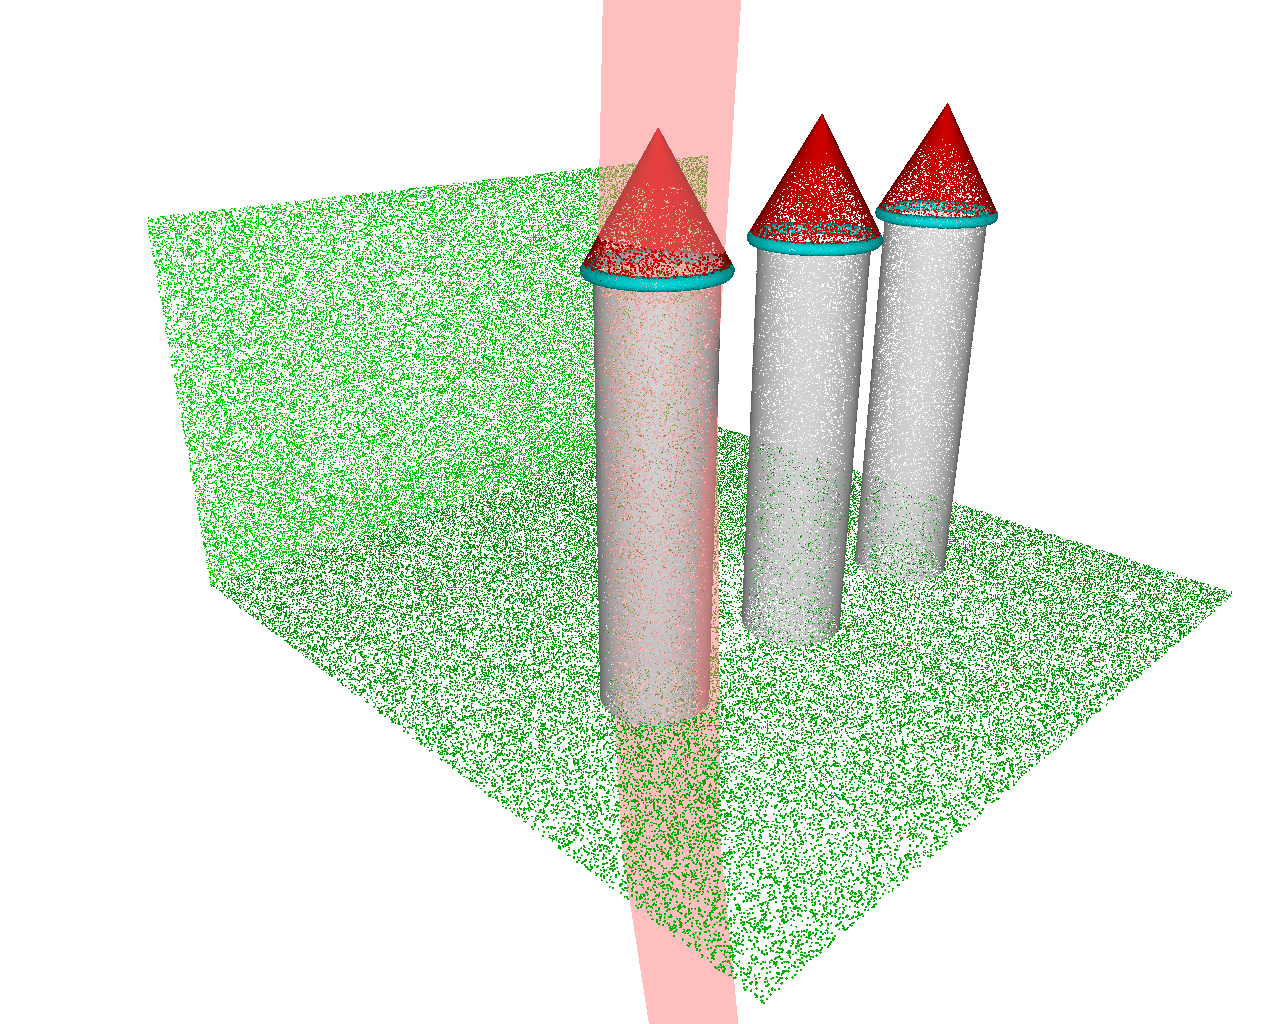
\includegraphics[width=0.49\textwidth]{Results/missfittedTorus1.png}%7
  }%\par\medskip
\subcaptionbox{ \label{fig:missfittedTorus2}}{%
  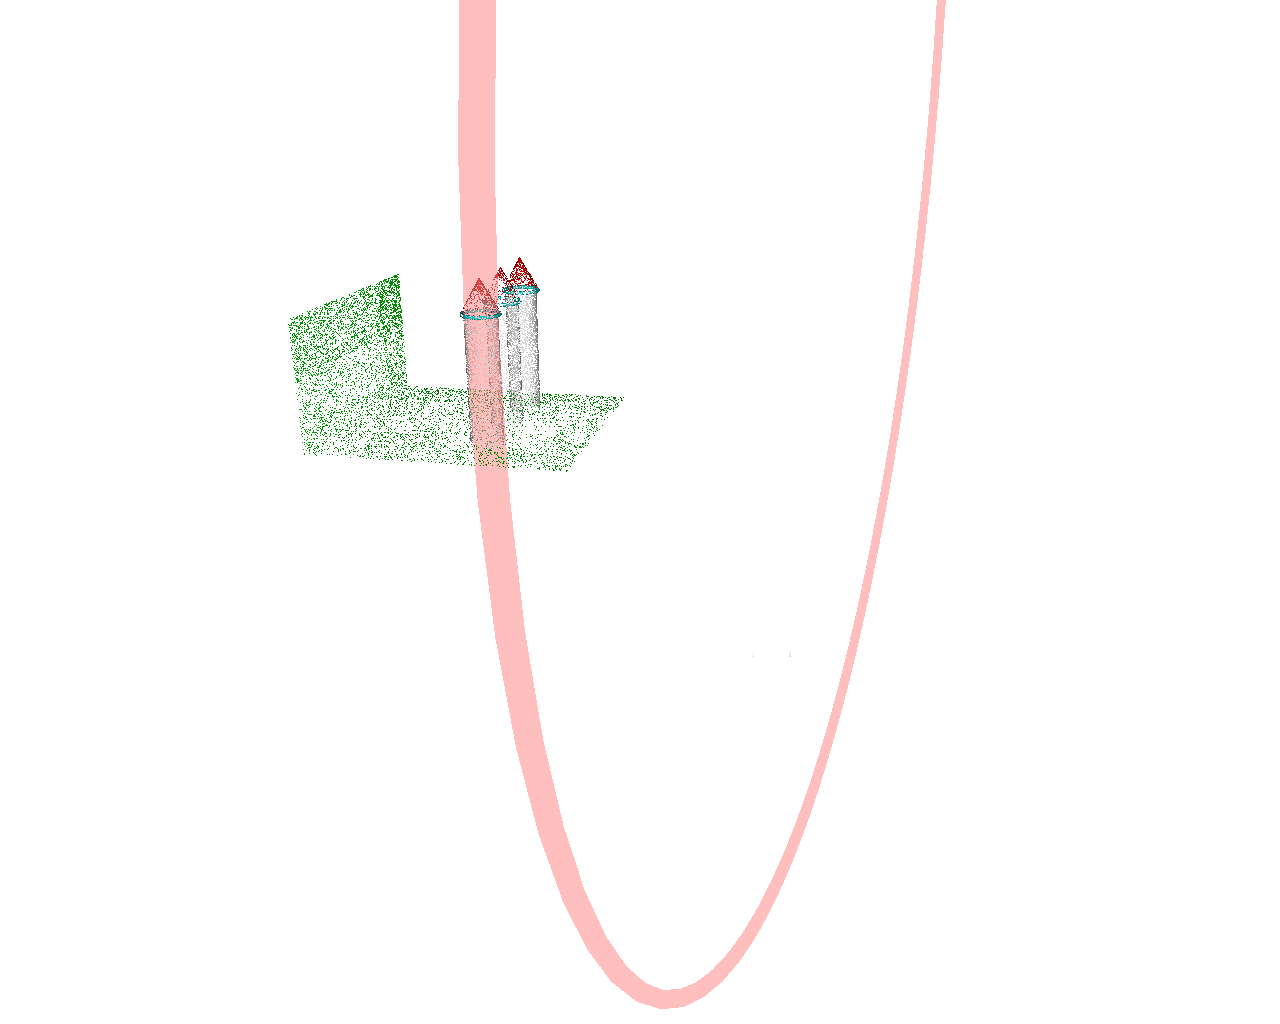
\includegraphics[width=0.49\textwidth]{Results/missfittedTorus2.png}%
  }    

  
\caption{This figure shows a synthesized cylinder in the foreground whose points are classified as a torus instead of a cylinder. Eventough the points fit the torus, determined by the RANSAC options, the result is not plausible, since the user would expect a cylinder for this constellation of points. }
\label{fig:missfittedTorus}
\end{figure}